% Options for packages loaded elsewhere
% Options for packages loaded elsewhere
\PassOptionsToPackage{unicode}{hyperref}
\PassOptionsToPackage{hyphens}{url}
\PassOptionsToPackage{dvipsnames,svgnames,x11names}{xcolor}
%
\documentclass[
  letterpaper,
  DIV=11,
  numbers=noendperiod]{scrartcl}
\usepackage{xcolor}
\usepackage{amsmath,amssymb}
\setcounter{secnumdepth}{-\maxdimen} % remove section numbering
\usepackage{iftex}
\ifPDFTeX
  \usepackage[T1]{fontenc}
  \usepackage[utf8]{inputenc}
  \usepackage{textcomp} % provide euro and other symbols
\else % if luatex or xetex
  \usepackage{unicode-math} % this also loads fontspec
  \defaultfontfeatures{Scale=MatchLowercase}
  \defaultfontfeatures[\rmfamily]{Ligatures=TeX,Scale=1}
\fi
\usepackage{lmodern}
\ifPDFTeX\else
  % xetex/luatex font selection
\fi
% Use upquote if available, for straight quotes in verbatim environments
\IfFileExists{upquote.sty}{\usepackage{upquote}}{}
\IfFileExists{microtype.sty}{% use microtype if available
  \usepackage[]{microtype}
  \UseMicrotypeSet[protrusion]{basicmath} % disable protrusion for tt fonts
}{}
\makeatletter
\@ifundefined{KOMAClassName}{% if non-KOMA class
  \IfFileExists{parskip.sty}{%
    \usepackage{parskip}
  }{% else
    \setlength{\parindent}{0pt}
    \setlength{\parskip}{6pt plus 2pt minus 1pt}}
}{% if KOMA class
  \KOMAoptions{parskip=half}}
\makeatother
% Make \paragraph and \subparagraph free-standing
\makeatletter
\ifx\paragraph\undefined\else
  \let\oldparagraph\paragraph
  \renewcommand{\paragraph}{
    \@ifstar
      \xxxParagraphStar
      \xxxParagraphNoStar
  }
  \newcommand{\xxxParagraphStar}[1]{\oldparagraph*{#1}\mbox{}}
  \newcommand{\xxxParagraphNoStar}[1]{\oldparagraph{#1}\mbox{}}
\fi
\ifx\subparagraph\undefined\else
  \let\oldsubparagraph\subparagraph
  \renewcommand{\subparagraph}{
    \@ifstar
      \xxxSubParagraphStar
      \xxxSubParagraphNoStar
  }
  \newcommand{\xxxSubParagraphStar}[1]{\oldsubparagraph*{#1}\mbox{}}
  \newcommand{\xxxSubParagraphNoStar}[1]{\oldsubparagraph{#1}\mbox{}}
\fi
\makeatother

\usepackage{color}
\usepackage{fancyvrb}
\newcommand{\VerbBar}{|}
\newcommand{\VERB}{\Verb[commandchars=\\\{\}]}
\DefineVerbatimEnvironment{Highlighting}{Verbatim}{commandchars=\\\{\}}
% Add ',fontsize=\small' for more characters per line
\usepackage{framed}
\definecolor{shadecolor}{RGB}{241,243,245}
\newenvironment{Shaded}{\begin{snugshade}}{\end{snugshade}}
\newcommand{\AlertTok}[1]{\textcolor[rgb]{0.68,0.00,0.00}{#1}}
\newcommand{\AnnotationTok}[1]{\textcolor[rgb]{0.37,0.37,0.37}{#1}}
\newcommand{\AttributeTok}[1]{\textcolor[rgb]{0.40,0.45,0.13}{#1}}
\newcommand{\BaseNTok}[1]{\textcolor[rgb]{0.68,0.00,0.00}{#1}}
\newcommand{\BuiltInTok}[1]{\textcolor[rgb]{0.00,0.23,0.31}{#1}}
\newcommand{\CharTok}[1]{\textcolor[rgb]{0.13,0.47,0.30}{#1}}
\newcommand{\CommentTok}[1]{\textcolor[rgb]{0.37,0.37,0.37}{#1}}
\newcommand{\CommentVarTok}[1]{\textcolor[rgb]{0.37,0.37,0.37}{\textit{#1}}}
\newcommand{\ConstantTok}[1]{\textcolor[rgb]{0.56,0.35,0.01}{#1}}
\newcommand{\ControlFlowTok}[1]{\textcolor[rgb]{0.00,0.23,0.31}{\textbf{#1}}}
\newcommand{\DataTypeTok}[1]{\textcolor[rgb]{0.68,0.00,0.00}{#1}}
\newcommand{\DecValTok}[1]{\textcolor[rgb]{0.68,0.00,0.00}{#1}}
\newcommand{\DocumentationTok}[1]{\textcolor[rgb]{0.37,0.37,0.37}{\textit{#1}}}
\newcommand{\ErrorTok}[1]{\textcolor[rgb]{0.68,0.00,0.00}{#1}}
\newcommand{\ExtensionTok}[1]{\textcolor[rgb]{0.00,0.23,0.31}{#1}}
\newcommand{\FloatTok}[1]{\textcolor[rgb]{0.68,0.00,0.00}{#1}}
\newcommand{\FunctionTok}[1]{\textcolor[rgb]{0.28,0.35,0.67}{#1}}
\newcommand{\ImportTok}[1]{\textcolor[rgb]{0.00,0.46,0.62}{#1}}
\newcommand{\InformationTok}[1]{\textcolor[rgb]{0.37,0.37,0.37}{#1}}
\newcommand{\KeywordTok}[1]{\textcolor[rgb]{0.00,0.23,0.31}{\textbf{#1}}}
\newcommand{\NormalTok}[1]{\textcolor[rgb]{0.00,0.23,0.31}{#1}}
\newcommand{\OperatorTok}[1]{\textcolor[rgb]{0.37,0.37,0.37}{#1}}
\newcommand{\OtherTok}[1]{\textcolor[rgb]{0.00,0.23,0.31}{#1}}
\newcommand{\PreprocessorTok}[1]{\textcolor[rgb]{0.68,0.00,0.00}{#1}}
\newcommand{\RegionMarkerTok}[1]{\textcolor[rgb]{0.00,0.23,0.31}{#1}}
\newcommand{\SpecialCharTok}[1]{\textcolor[rgb]{0.37,0.37,0.37}{#1}}
\newcommand{\SpecialStringTok}[1]{\textcolor[rgb]{0.13,0.47,0.30}{#1}}
\newcommand{\StringTok}[1]{\textcolor[rgb]{0.13,0.47,0.30}{#1}}
\newcommand{\VariableTok}[1]{\textcolor[rgb]{0.07,0.07,0.07}{#1}}
\newcommand{\VerbatimStringTok}[1]{\textcolor[rgb]{0.13,0.47,0.30}{#1}}
\newcommand{\WarningTok}[1]{\textcolor[rgb]{0.37,0.37,0.37}{\textit{#1}}}

\usepackage{longtable,booktabs,array}
\newcounter{none} % for unnumbered tables
\usepackage{calc} % for calculating minipage widths
% Correct order of tables after \paragraph or \subparagraph
\usepackage{etoolbox}
\makeatletter
\patchcmd\longtable{\par}{\if@noskipsec\mbox{}\fi\par}{}{}
\makeatother
% Allow footnotes in longtable head/foot
\IfFileExists{footnotehyper.sty}{\usepackage{footnotehyper}}{\usepackage{footnote}}
\makesavenoteenv{longtable}
\usepackage{graphicx}
\makeatletter
\newsavebox\pandoc@box
\newcommand*\pandocbounded[1]{% scales image to fit in text height/width
  \sbox\pandoc@box{#1}%
  \Gscale@div\@tempa{\textheight}{\dimexpr\ht\pandoc@box+\dp\pandoc@box\relax}%
  \Gscale@div\@tempb{\linewidth}{\wd\pandoc@box}%
  \ifdim\@tempb\p@<\@tempa\p@\let\@tempa\@tempb\fi% select the smaller of both
  \ifdim\@tempa\p@<\p@\scalebox{\@tempa}{\usebox\pandoc@box}%
  \else\usebox{\pandoc@box}%
  \fi%
}
% Set default figure placement to htbp
\def\fps@figure{htbp}
\makeatother





\setlength{\emergencystretch}{3em} % prevent overfull lines

\providecommand{\tightlist}{%
  \setlength{\itemsep}{0pt}\setlength{\parskip}{0pt}}



 


\KOMAoption{captions}{tableheading}
\makeatletter
\@ifpackageloaded{caption}{}{\usepackage{caption}}
\AtBeginDocument{%
\ifdefined\contentsname
  \renewcommand*\contentsname{Table of contents}
\else
  \newcommand\contentsname{Table of contents}
\fi
\ifdefined\listfigurename
  \renewcommand*\listfigurename{List of Figures}
\else
  \newcommand\listfigurename{List of Figures}
\fi
\ifdefined\listtablename
  \renewcommand*\listtablename{List of Tables}
\else
  \newcommand\listtablename{List of Tables}
\fi
\ifdefined\figurename
  \renewcommand*\figurename{Figure}
\else
  \newcommand\figurename{Figure}
\fi
\ifdefined\tablename
  \renewcommand*\tablename{Table}
\else
  \newcommand\tablename{Table}
\fi
}
\@ifpackageloaded{float}{}{\usepackage{float}}
\floatstyle{ruled}
\@ifundefined{c@chapter}{\newfloat{codelisting}{h}{lop}}{\newfloat{codelisting}{h}{lop}[chapter]}
\floatname{codelisting}{Listing}
\newcommand*\listoflistings{\listof{codelisting}{List of Listings}}
\makeatother
\makeatletter
\makeatother
\makeatletter
\@ifpackageloaded{caption}{}{\usepackage{caption}}
\@ifpackageloaded{subcaption}{}{\usepackage{subcaption}}
\makeatother
\usepackage{bookmark}
\IfFileExists{xurl.sty}{\usepackage{xurl}}{} % add URL line breaks if available
\urlstyle{same}
% fallback for those not using the hyperref driver hyperxmp:
\makeatletter
\@ifundefined{xmpquote}{\newcommand{\xmpquote}[1]{#1}}{}
\makeatother
\hypersetup{
  pdftitle={Week 7},
  colorlinks=true,
  linkcolor={blue},
  filecolor={Maroon},
  citecolor={Blue},
  urlcolor={Blue},
  pdfcreator={LaTeX via pandoc}}


\title{Week 7}
\author{}
\date{}
\begin{document}
\maketitle


\section{Regression with categorical
predictors}\label{regression-with-categorical-predictors}

Previously we have fitted regression models of the following form in R
using brms:

\(y∼Gaussian(\mu, \sigma)\)

\(\mu = \beta_0 + \beta_1 ⋅ x\)

Here, x was a numeric predictor like speech rate. They are not the only
type of predictors. They can have categorical variables like gender or
age group. They cant handle a categorical predictor directly you cant
multiply \(\beta_1\) by female. We have to recode them as numbers.

In this chapter we will revisit the MALD reaction times (RTs) data from
\href{https://stefanocoretta.github.io/qdal/ch-fit-model.html}{Chapter
22}, this time with the following research question:

\begin{quote}
Is the RTs in a auditory lexical decision task affected by the type of
the target word (real or not)?
\end{quote}

\begin{Shaded}
\begin{Highlighting}[]
\FunctionTok{library}\NormalTok{(tidyverse)}
\end{Highlighting}
\end{Shaded}

\begin{verbatim}
Warning: package 'tidyverse' was built under R version 4.5.3
\end{verbatim}

\begin{verbatim}
Warning: package 'ggplot2' was built under R version 4.5.3
\end{verbatim}

\begin{verbatim}
Warning: package 'tidyr' was built under R version 4.5.3
\end{verbatim}

\begin{verbatim}
Warning: package 'readr' was built under R version 4.5.3
\end{verbatim}

\begin{verbatim}
Warning: package 'purrr' was built under R version 4.5.3
\end{verbatim}

\begin{verbatim}
Warning: package 'forcats' was built under R version 4.5.3
\end{verbatim}

\begin{verbatim}
Warning: package 'lubridate' was built under R version 4.5.3
\end{verbatim}

\begin{verbatim}
-- Attaching core tidyverse packages ------------------------ tidyverse 2.0.0 --
v dplyr     1.2.0     v readr     2.2.0
v forcats   1.0.1     v stringr   1.6.0
v ggplot2   4.0.2     v tibble    3.3.1
v lubridate 1.9.5     v tidyr     1.3.2
v purrr     1.2.1     
-- Conflicts ------------------------------------------ tidyverse_conflicts() --
x dplyr::filter() masks stats::filter()
x dplyr::lag()    masks stats::lag()
i Use the conflicted package (<http://conflicted.r-lib.org/>) to force all conflicts to become errors
\end{verbatim}

\begin{Shaded}
\begin{Highlighting}[]
\FunctionTok{theme\_set}\NormalTok{(}\FunctionTok{theme\_light}\NormalTok{())}
\FunctionTok{library}\NormalTok{(brms)}
\end{Highlighting}
\end{Shaded}

\begin{verbatim}
Warning: package 'brms' was built under R version 4.5.3
\end{verbatim}

\begin{verbatim}
Loading required package: Rcpp
\end{verbatim}

\begin{verbatim}
Warning: package 'Rcpp' was built under R version 4.5.3
\end{verbatim}

\begin{verbatim}
Loading 'brms' package (version 2.23.0). Useful instructions
can be found by typing help('brms'). A more detailed introduction
to the package is available through vignette('brms_overview').

Attaching package: 'brms'

The following object is masked from 'package:stats':

    ar
\end{verbatim}

\begin{Shaded}
\begin{Highlighting}[]
\FunctionTok{library}\NormalTok{(posterior)}
\end{Highlighting}
\end{Shaded}

\begin{verbatim}
Warning: package 'posterior' was built under R version 4.5.3
\end{verbatim}

\begin{verbatim}
This is posterior version 1.7.0

Attaching package: 'posterior'

The following objects are masked from 'package:stats':

    mad, sd, var

The following objects are masked from 'package:base':

    %in%, match
\end{verbatim}

\begin{Shaded}
\begin{Highlighting}[]
\FunctionTok{library}\NormalTok{(bayesplot)}
\end{Highlighting}
\end{Shaded}

\begin{verbatim}
Warning: package 'bayesplot' was built under R version 4.5.3
\end{verbatim}

\begin{verbatim}
This is bayesplot version 1.16.0
- Online documentation and vignettes at mc-stan.org/bayesplot
- bayesplot theme set to bayesplot::theme_default()
   * Does _not_ affect other ggplot2 plots
   * See ?bayesplot_theme_set for details on theme setting

Attaching package: 'bayesplot'

The following object is masked from 'package:posterior':

    rhat

The following object is masked from 'package:brms':

    rhat
\end{verbatim}

\begin{Shaded}
\begin{Highlighting}[]
\FunctionTok{library}\NormalTok{(ggdist)}
\end{Highlighting}
\end{Shaded}

\begin{verbatim}
Warning: package 'ggdist' was built under R version 4.5.3
\end{verbatim}

\begin{verbatim}

Attaching package: 'ggdist'

The following objects are masked from 'package:brms':

    dstudent_t, pstudent_t, qstudent_t, rstudent_t
\end{verbatim}

\begin{Shaded}
\begin{Highlighting}[]
\NormalTok{mald }\OtherTok{\textless{}{-}} \FunctionTok{readRDS}\NormalTok{(}\StringTok{"./data/tucker2019/mald\_1\_1.rds"}\NormalTok{)}

\NormalTok{mald}
\end{Highlighting}
\end{Shaded}

\begin{verbatim}
# A tibble: 5,000 x 8
   Subject Item        IsWord PhonLev FreqSUBTLEX    RT ACC     RT_log
   <chr>   <chr>       <fct>    <dbl>       <dbl> <int> <fct>    <dbl>
 1 15308   acreage     TRUE      6.01          22   617 correct   6.42
 2 15308   maxraezaxr  FALSE     6.78           0  1198 correct   7.09
 3 15308   prognosis   TRUE      8.14          54   954 correct   6.86
 4 15308   giggles     TRUE      6.22         170   579 correct   6.36
 5 15308   baazh       FALSE     6.13           0  1011 correct   6.92
 6 15308   unflagging  TRUE      7.66           4  1402 correct   7.25
 7 15308   ihnpaykaxrz FALSE     7.47           0  1059 correct   6.97
 8 15308   hawk        TRUE      6.09         650   739 correct   6.61
 9 15308   assessing   TRUE      6.37          27   789 correct   6.67
10 15308   mehlaxl     FALSE     5.80           0   926 correct   6.83
# i 4,990 more rows
\end{verbatim}

Here we are interested in the RT and IsWord \texttt{TRUE} or
\texttt{FALSE}. We can cerate a density plot of RTs:

\begin{Shaded}
\begin{Highlighting}[]
\NormalTok{mald }\SpecialCharTok{|\textgreater{}}
  \FunctionTok{ggplot}\NormalTok{(}\FunctionTok{aes}\NormalTok{(RT, }\AttributeTok{fill =}\NormalTok{ IsWord)) }\SpecialCharTok{+}
  \FunctionTok{geom\_density}\NormalTok{(}\AttributeTok{alpha =} \FloatTok{0.8}\NormalTok{) }\SpecialCharTok{+}
  \FunctionTok{geom\_rug}\NormalTok{(}\AttributeTok{alpha =} \FloatTok{0.1}\NormalTok{) }\SpecialCharTok{+}
  \FunctionTok{scale\_fill\_brewer}\NormalTok{(}\AttributeTok{palette =} \StringTok{"Dark2"}\NormalTok{) }
\end{Highlighting}
\end{Shaded}

\pandocbounded{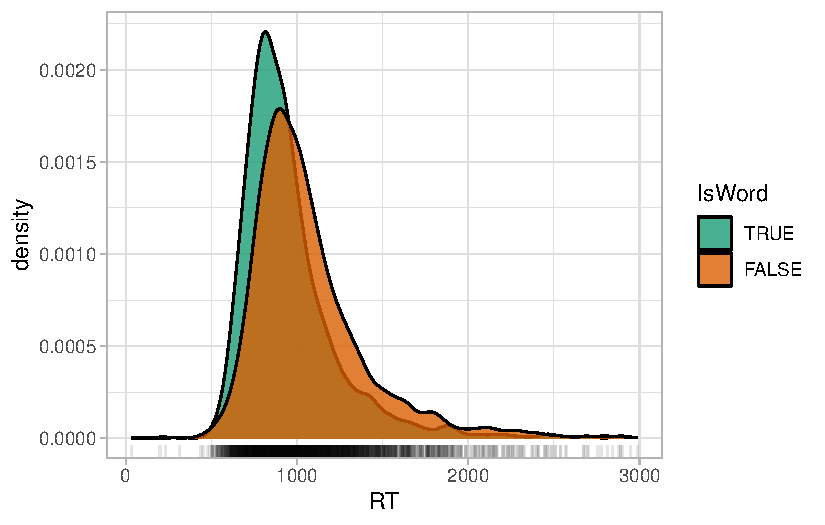
\includegraphics[keepaspectratio]{week-7_files/figure-pdf/unnamed-chunk-3-1.pdf}}

You might also notice that the ``tails'' of the distributions (the left
and right sides) are not symmetric: the right tail is heavier that the
left tail. This is a very common characteristics of RT values and of any
variable that can only be positive (like vowel duration or the duration
of any other phonetic unit). These variables are ``bounded'' to only
positive numbers. You will learn later on that the values in these
variables are generated by a log-normal distribution
(\href{https://stefanocoretta.github.io/qdal/ch-regression-lognorm.html}{Chapter
32}), rather than by a Gaussian distribution (which is ``unbounded'').
For the time being though, we will model the data as if they were
generated by a Gaussian distribution, so that we can focus on the
categorical predictor part.

We can also use a jitter plot to present numeric variables that depend
on categorical variables. The width of the strips can be adjusted using
the \texttt{width} argument. These are two ways of visualising the same
thing:

\begin{Shaded}
\begin{Highlighting}[]
\NormalTok{mald }\SpecialCharTok{|\textgreater{}}
  \FunctionTok{ggplot}\NormalTok{(}\FunctionTok{aes}\NormalTok{(IsWord, RT, }\AttributeTok{colour =}\NormalTok{ IsWord)) }\SpecialCharTok{+} 
  \CommentTok{\#width argument}
  \FunctionTok{geom\_jitter}\NormalTok{(}\AttributeTok{alpha =} \FloatTok{0.15}\NormalTok{, }\AttributeTok{width =} \FloatTok{0.13}\NormalTok{) }\SpecialCharTok{+} 
  \FunctionTok{scale\_colour\_brewer}\NormalTok{(}\AttributeTok{palette =} \StringTok{"Dark2"}\NormalTok{)}
\end{Highlighting}
\end{Shaded}

\pandocbounded{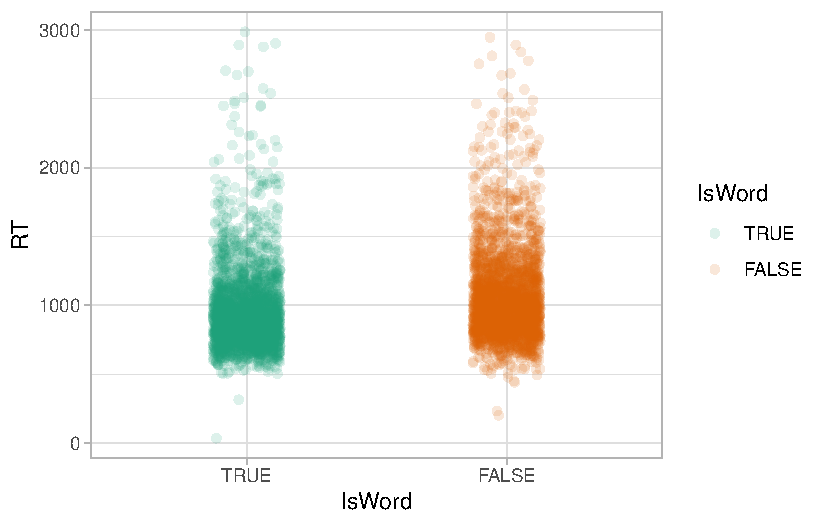
\includegraphics[keepaspectratio]{week-7_files/figure-pdf/unnamed-chunk-4-1.pdf}}

You can also overlay a density plot on the jitter plot using
\texttt{geom\_violin}. \texttt{width} also works for the violin and
jitter, independently.

\begin{Shaded}
\begin{Highlighting}[]
\NormalTok{mald }\SpecialCharTok{|\textgreater{}}
  \FunctionTok{ggplot}\NormalTok{(}\FunctionTok{aes}\NormalTok{(IsWord, RT, }\AttributeTok{fill =}\NormalTok{ IsWord)) }\SpecialCharTok{+} 
  \FunctionTok{geom\_jitter}\NormalTok{(}\AttributeTok{alpha =} \FloatTok{0.5}\NormalTok{, }\AttributeTok{width =} \FloatTok{0.13}\NormalTok{) }\SpecialCharTok{+}
  \FunctionTok{geom\_violin}\NormalTok{(}\AttributeTok{width =} \FloatTok{0.26}\NormalTok{) }\SpecialCharTok{+} 
  \FunctionTok{scale\_fill\_brewer}\NormalTok{(}\AttributeTok{palette =} \StringTok{"Dark2"}\NormalTok{)}
\end{Highlighting}
\end{Shaded}

\pandocbounded{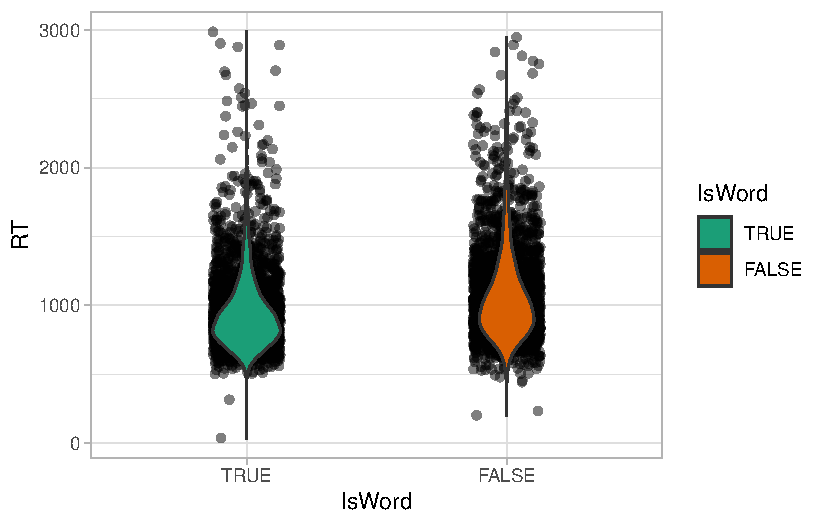
\includegraphics[keepaspectratio]{week-7_files/figure-pdf/unnamed-chunk-5-1.pdf}}

\textbf{Data that combines one numeric and one or more categorical
variables can be represented with jitter and violin plots}.

\begin{Shaded}
\begin{Highlighting}[]
\NormalTok{mald }\SpecialCharTok{|\textgreater{}}
  \FunctionTok{ggplot}\NormalTok{(}\FunctionTok{aes}\NormalTok{(IsWord, RT, }\AttributeTok{fill =}\NormalTok{ IsWord)) }\SpecialCharTok{+}
  \FunctionTok{geom\_violin}\NormalTok{(}\AttributeTok{width =} \FloatTok{0.2}\NormalTok{) }\SpecialCharTok{+} 
  \FunctionTok{scale\_fill\_brewer}\NormalTok{(}\AttributeTok{palette =} \StringTok{"Dark2"}\NormalTok{)}
\end{Highlighting}
\end{Shaded}

\pandocbounded{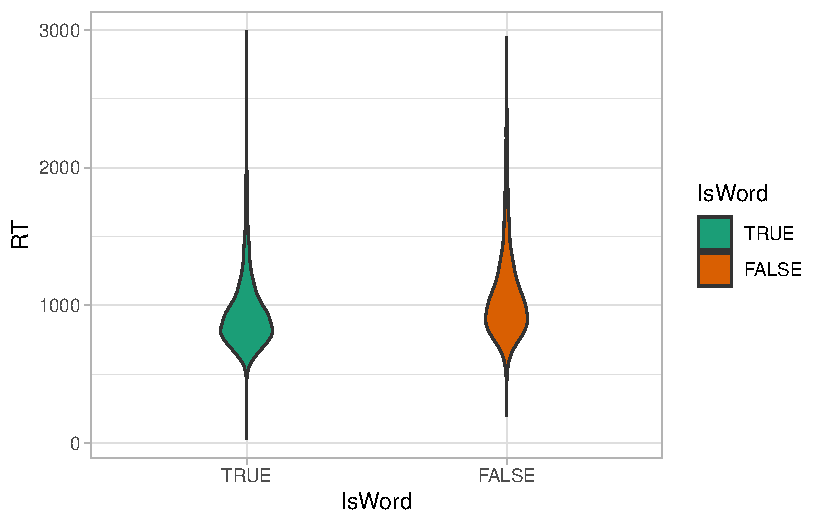
\includegraphics[keepaspectratio]{week-7_files/figure-pdf/unnamed-chunk-6-1.pdf}}

It is good practice to show the raw data and the density using violin
and jitter plots, because patterns in the data are visible when plotting
the raw data (while they aren't when using for example bar charts, more
on this in
\href{https://stefanocoretta.github.io/qdal/ch-regression-bernoulli.html\#sec-plot-prop}{Section
30.3}), so this should be your go-to choice for plotting numeric data by
categorical groups, like RTs and type of word here. Now we can obtain a
few summary measures. The following code groups the data by
\texttt{IsWord} and then calculates the mean, median and standard
deviation of RTs. After \texttt{summarise()}, we are using a trick to
round all columns that are numeric, namely the columns with the mean,
median and SD. The trick is to use the \texttt{across()} function in
combination of \texttt{where()}.
\texttt{across(where(is.numeric),\ round)} means ``\emph{across} columns
where the type \emph{is numeric}, \emph{round} the value''.

\begin{Shaded}
\begin{Highlighting}[]
\NormalTok{mald\_summ }\OtherTok{\textless{}{-}}\NormalTok{ mald }\SpecialCharTok{|\textgreater{}} 
  \FunctionTok{group\_by}\NormalTok{(IsWord) }\SpecialCharTok{|\textgreater{}} 
  \FunctionTok{summarise}\NormalTok{(}
    \FunctionTok{mean}\NormalTok{(RT), }\FunctionTok{median}\NormalTok{(RT), }\FunctionTok{sd}\NormalTok{(RT)}
\NormalTok{  ) }\SpecialCharTok{|\textgreater{}} 
  \FunctionTok{mutate}\NormalTok{(}
    \CommentTok{\# round all numeric columns}
    \FunctionTok{across}\NormalTok{(}\FunctionTok{where}\NormalTok{(is.numeric), round)}
\NormalTok{  )}

\NormalTok{mald\_summ}
\end{Highlighting}
\end{Shaded}

\begin{verbatim}
# A tibble: 2 x 4
  IsWord `mean(RT)` `median(RT)` `sd(RT)`
  <fct>       <dbl>        <dbl>    <dbl>
1 TRUE          953          888      291
2 FALSE        1069          994      333
\end{verbatim}

The mean and median RTs for non-words are about 100 ms higher than the
mean and median of real words. If we stopped here we wouldnt be covering
uncertainty and variability. With a sample of this size we should apply
inference from the sample to the population to obtain an estimate of the
difference in RTs that accounts for uncertainty and variability. We can
use regression models to do this.

\section{\texorpdfstring{\texttt{kable()}}{kable()}}\label{kable}

You can output summaries as a table, using \texttt{knittr::kable()}:

\begin{Shaded}
\begin{Highlighting}[]
\NormalTok{knitr}\SpecialCharTok{::}\FunctionTok{kable}\NormalTok{(}
\NormalTok{  mald\_summ,}
  \AttributeTok{digits =} \DecValTok{0}\NormalTok{, }\AttributeTok{col.names =} \FunctionTok{c}\NormalTok{(}\StringTok{"Is word?"}\NormalTok{, }\StringTok{"mean"}\NormalTok{, }\StringTok{"median"}\NormalTok{, }\StringTok{"SD"}\NormalTok{) }
\NormalTok{)}
\end{Highlighting}
\end{Shaded}

{\def\LTcaptype{none} % do not increment counter
\begin{longtable}[]{@{}lrrr@{}}
\toprule\noalign{}
Is word? & mean & median & SD \\
\midrule\noalign{}
\endhead
\bottomrule\noalign{}
\endlastfoot
TRUE & 953 & 888 & 291 \\
FALSE & 1069 & 994 & 333 \\
\end{longtable}
}

\section{Treatment Contrasts}\label{treatment-contrasts}

We can model the RTs with a Gaussian dist. (this family isnt usually
appropriate for variables like RTs). with a mean and SD where
\(RT∼Gaussian(\mu,\sigma)\). This time we want to model a different
\(/mu\) depending on the word type in \texttt{IsWord}. We can do this in
seevral ways. The default is called \textbf{treatment contrasts} which
involves numerical coding of categorical predictors. Using IsWord as an
example, it is a categorical predictor with two levels \texttt{TRUE} and
\texttt{FALSE}. with treatment contrasts one level is chosen as a
\textbf{reference level} and the other one is compared to it. The
reference level is automatically set as the first level in the predictor
in alphabetical order. This would mean that \texttt{FALSE} would be the
reference level.

However, in the mald data, the column IsWord is a factor column and the
levels have been ordered so that TRUE is the first level and FALSE the
second. You can see this in the Environment panel, if you click on the
arrow next to mald and look next to IsWord: it will say Factor w/ 2
levels ``TRUE'',``FALSE''. You can also check the order of the levels of
a factor with the levels() function.

\begin{Shaded}
\begin{Highlighting}[]
\FunctionTok{levels}\NormalTok{(mald}\SpecialCharTok{$}\NormalTok{IsWord)}
\end{Highlighting}
\end{Shaded}

\begin{verbatim}
[1] "TRUE"  "FALSE"
\end{verbatim}

We can set the order ourselves with \texttt{factor()}.

\begin{Shaded}
\begin{Highlighting}[]
\NormalTok{fac }\OtherTok{\textless{}{-}} \FunctionTok{tibble}\NormalTok{(}
  \AttributeTok{fac =} \FunctionTok{c}\NormalTok{(}\StringTok{"a"}\NormalTok{, }\StringTok{"a"}\NormalTok{, }\StringTok{"b"}\NormalTok{, }\StringTok{"b"}\NormalTok{, }\StringTok{"a"}\NormalTok{),}
  \AttributeTok{fac\_1 =} \FunctionTok{factor}\NormalTok{(fac),}
  \AttributeTok{fac\_2 =} \FunctionTok{factor}\NormalTok{(fac, }\AttributeTok{levels =} \FunctionTok{c}\NormalTok{(}\StringTok{"b"}\NormalTok{, }\StringTok{"a"}\NormalTok{))}
\NormalTok{)}

\FunctionTok{levels}\NormalTok{(fac}\SpecialCharTok{$}\NormalTok{fac\_1)}
\end{Highlighting}
\end{Shaded}

\begin{verbatim}
[1] "a" "b"
\end{verbatim}

\begin{Shaded}
\begin{Highlighting}[]
\FunctionTok{levels}\NormalTok{(fac}\SpecialCharTok{$}\NormalTok{fac\_2)}
\end{Highlighting}
\end{Shaded}

\begin{verbatim}
[1] "b" "a"
\end{verbatim}

We will use IsWord with the order TRUE and FALSE. This means that TRUE
will be the reference level and the RTs when IsWord is FALSE will be
compared to the RTs of when IsWord is TRUE. In other words, now the mean
𝜇 varies depending on the level of IsWord. We need to numerically code
IsWord (i.e.~use numbers to refer to the levels of the categorical
predictor) to be able to allow the mean to vary by the word type in the
model formula. With treatment contrasts, treatment coding is used to
numerically code categorical predictors. Treatment coding uses indicator
variables which take the values 0 or 1. Let's make an indicator variable
𝑤 that is 0 when IsWord is TRUE, or 1 when IsWord is FALSE. We only need
one indicator variable because there are only two levels and they can be
coded with a 0 and a 1 respectively. This way of setting up indicator
variables (using 0/1) is called dummy coding. See Table 28.2 for the
correspondence between the predictor IsWord and the value of the
indicator variable 𝑤.

{\def\LTcaptype{none} % do not increment counter
\begin{longtable}[]{@{}ll@{}}
\toprule\noalign{}
\endhead
\bottomrule\noalign{}
\endlastfoot
\texttt{IsWord} & \(w\) \\
IsWord = TRUE & 0 \\
IsWord = False & 1 \\
\end{longtable}
}

We can now update the equation of \(\mu\)

\(RT_i ∼ Gaussian(\mu_i,\sigma)\)

\(\mu_i = \beta_0 + \beta_1 ⋅sr_i\)

Going back to our model of RTs as a function of word type (``as a
function of'' is another way of saying that you are modelling an outcome
variable depending on a predictor), 𝛽0 and 𝛽1 are the regression
coefficients, exactly like in the regression model with vowel duration
and speech rate. You can think of 𝛽0 as the model's intercept and of 𝛽1
as the model's slope. Can you figure out why? Recall that a regression
model with a numeric predictor is basically the formula of a line. In
\href{https://stefanocoretta.github.io/qdal/ch-regression.html}{Chapter
24}, we modelled vowel duration as a function of speech rate. The
intercept of the regression line estimated by the model indicates where
the line crosses the \emph{y}-axis when the \emph{x} value is 0: in that
model, that was the vowel duration when speech rate is 0. In the model
of RTs above, with RTs as a function of word type, the numeric predictor
is the indicator variable 𝑤, which stands for the categorical predictor
\texttt{IsWord}. The formula of a line really works just with numbers so
for the formula to make sense, we had to make the categorical predictor
\texttt{IsWord} into a number and treatment contrasts is such one way of
doing so.

Now, 𝛽0 is the model's intercept because that is the mean RT when 𝑤 is 0
(like with vowel duration when speech rate is 0; can you see the
parallel?). And 𝛽1 is the model's slope because 𝛽1 is the change in RT
for a unit increase of 𝑤, which is when 𝑤 goes from 0 to 1. This in turn
corresponds to the change in level in the categorical predictor. Do you
see the connection? It's a bit contorted, but once you get this, it
should explain several aspects of regression models with categorical
predictors and treatment contrasts. So 𝜇𝑖 is the sum of 𝛽0 and 𝛽1 ⋅𝑤𝑖.
𝑤𝑖 is 0 (when the word is real) or 1 (the the word is a non-word). That
is why we write 𝑅⁢𝑇𝑖: the subscript 𝑖 allows us to pick the correct value
of 𝑤𝑖 for each specific observation. The result of plugging in the value
of 𝑤𝑖 is laid out in the following formulae.

\pandocbounded{\includegraphics[keepaspectratio]{images/clipboard-1967116651.png}}

When IsWord is true the mean RT is = beta0

when it is false it is equal to beta0+beta1

is beta0 is the mean RT when isWord is true what is beta1 by itself

𝛽1=𝜇F−𝜇T=(𝛽0+𝛽1)−𝛽0

𝛽1 is the \emph{difference} between the mean RT when \texttt{IsWord} is
\texttt{TRUE} and the mean RT when \texttt{IsWord} is \texttt{FALSE}. As
mentioned above, with treatment contrasts you are comparing the second
level to the first. So one regression coefficient will be the mean of
the reference level, and the other coefficient will be the
\emph{difference} between the mean of the two levels. I know this is not
particularly beginner-friendly, but this is the default in R when using
categorical predictors and it is the most common way to code categorical
predictors, so you will frequently find tables in academic articles with
regression coefficients that have to be interpreted that way.

\section{Modelling RT by word type}\label{modelling-rt-by-word-type}

if we want to fit a model with a categorical predictor like IsWord we
jus tneed to include it in the formula to the right of the
\texttt{\textasciitilde{}}.

\begin{Shaded}
\begin{Highlighting}[]
\NormalTok{rt\_brm\_1 }\OtherTok{\textless{}{-}} \FunctionTok{brm}\NormalTok{(}
  \CommentTok{\#no need to inclue 1+ as it is included by default.}
\NormalTok{  RT }\SpecialCharTok{\textasciitilde{}}\NormalTok{ IsWord,}
  \AttributeTok{family =}\NormalTok{ gaussian, }
  \AttributeTok{data =}\NormalTok{ mald,}
  \AttributeTok{seed =} \DecValTok{6725}\NormalTok{,}
  \AttributeTok{file =} \StringTok{"cache/ch{-}regression{-}cat{-}rt\_bm\_1"}
\NormalTok{)}
\end{Highlighting}
\end{Shaded}

\begin{Shaded}
\begin{Highlighting}[]
\FunctionTok{summary}\NormalTok{(rt\_brm\_1)}
\end{Highlighting}
\end{Shaded}

\begin{verbatim}
 Family: gaussian 
  Links: mu = identity 
Formula: RT ~ IsWord 
   Data: mald (Number of observations: 5000) 
  Draws: 4 chains, each with iter = 2000; warmup = 1000; thin = 1;
         total post-warmup draws = 4000

Regression Coefficients:
            Estimate Est.Error l-95% CI u-95% CI Rhat Bulk_ESS Tail_ESS
Intercept     952.98      6.33   940.59   965.05 1.00     3991     2693
IsWordFALSE   116.16      9.08    98.00   133.58 1.00     3515     2920

Further Distributional Parameters:
      Estimate Est.Error l-95% CI u-95% CI Rhat Bulk_ESS Tail_ESS
sigma   312.63      3.12   306.69   318.94 1.00     3544     3031

Draws were sampled using sampling(NUTS). For each parameter, Bulk_ESS
and Tail_ESS are effective sample size measures, and Rhat is the potential
scale reduction factor on split chains (at convergence, Rhat = 1).
\end{verbatim}

\begin{Shaded}
\begin{Highlighting}[]
\FunctionTok{fixef}\NormalTok{(rt\_brm\_1) }\SpecialCharTok{|\textgreater{}} 
\NormalTok{  knitr}\SpecialCharTok{::}\FunctionTok{kable}\NormalTok{()}
\end{Highlighting}
\end{Shaded}

{\def\LTcaptype{none} % do not increment counter
\begin{longtable}[]{@{}lrrrr@{}}
\toprule\noalign{}
& Estimate & Est.Error & Q2.5 & Q97.5 \\
\midrule\noalign{}
\endhead
\bottomrule\noalign{}
\endlastfoot
Intercept & 952.9757 & 6.331974 & 940.58976 & 965.0485 \\
IsWordFALSE & 116.1620 & 9.081401 & 97.99835 & 133.5848 \\
\end{longtable}
}




\end{document}
